\subsection{Results on the DECam Survey}
\label{sec:results_on_decam}

We next demostrate StarNet on a larger region of the sky.
The DECam survey imaged stars in our own Milky Way, and we chose
a $4000 \times 2000$ frame centered at coordinates $\text{RA} = 266.044^\circ$ and
$\text{DEC} = -28.88111^\circ$. See Figure~\ref{fig:decaps} for an example image.

The DECam image is somewhat sparser than M2.
Thus, we set the Poisson mean parameter of the star density lower smaller than on M2 to fifty stars per $100 \times 100$-pixel image.
This allowed us to use larger $10\times 10$-pixel tiles with $20\times20$-pixel
padded tiles. 
We produced
a catalog for the full $4000 \times 1000$ frame, consisting of $9,000$ stars. 
The color-magnitude diagram shows a sequence of blue
stars that are reddened at fainter magnitudes. 

\begin{figure}[!htb]
    \centering
    \begin{subfigure}[T]{0.45\textwidth}
    \centering
    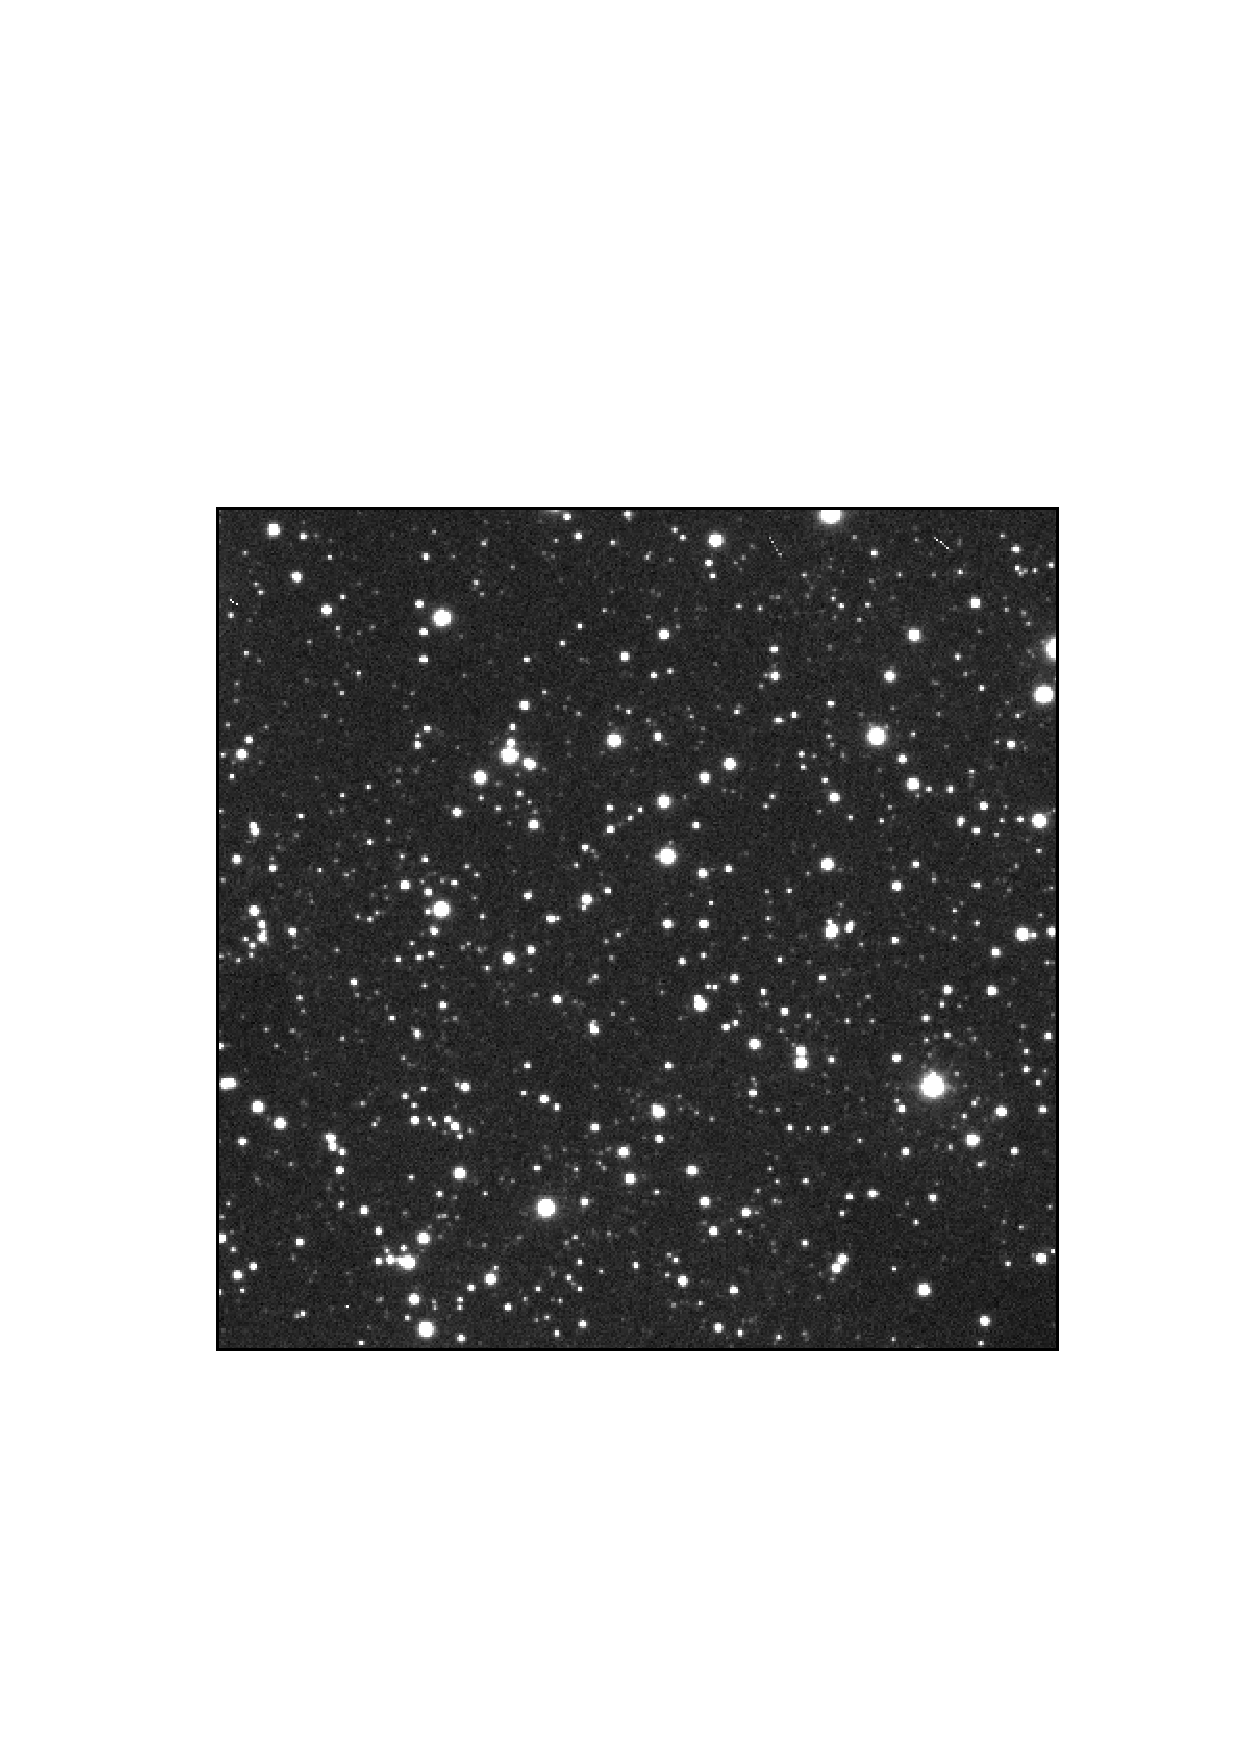
\includegraphics[width=\textwidth]{./figures/decaps/example_subimage1000_decaps.png}
    \end{subfigure}
    \hfill
    \begin{subfigure}[T]{0.5\textwidth}
    \centering
    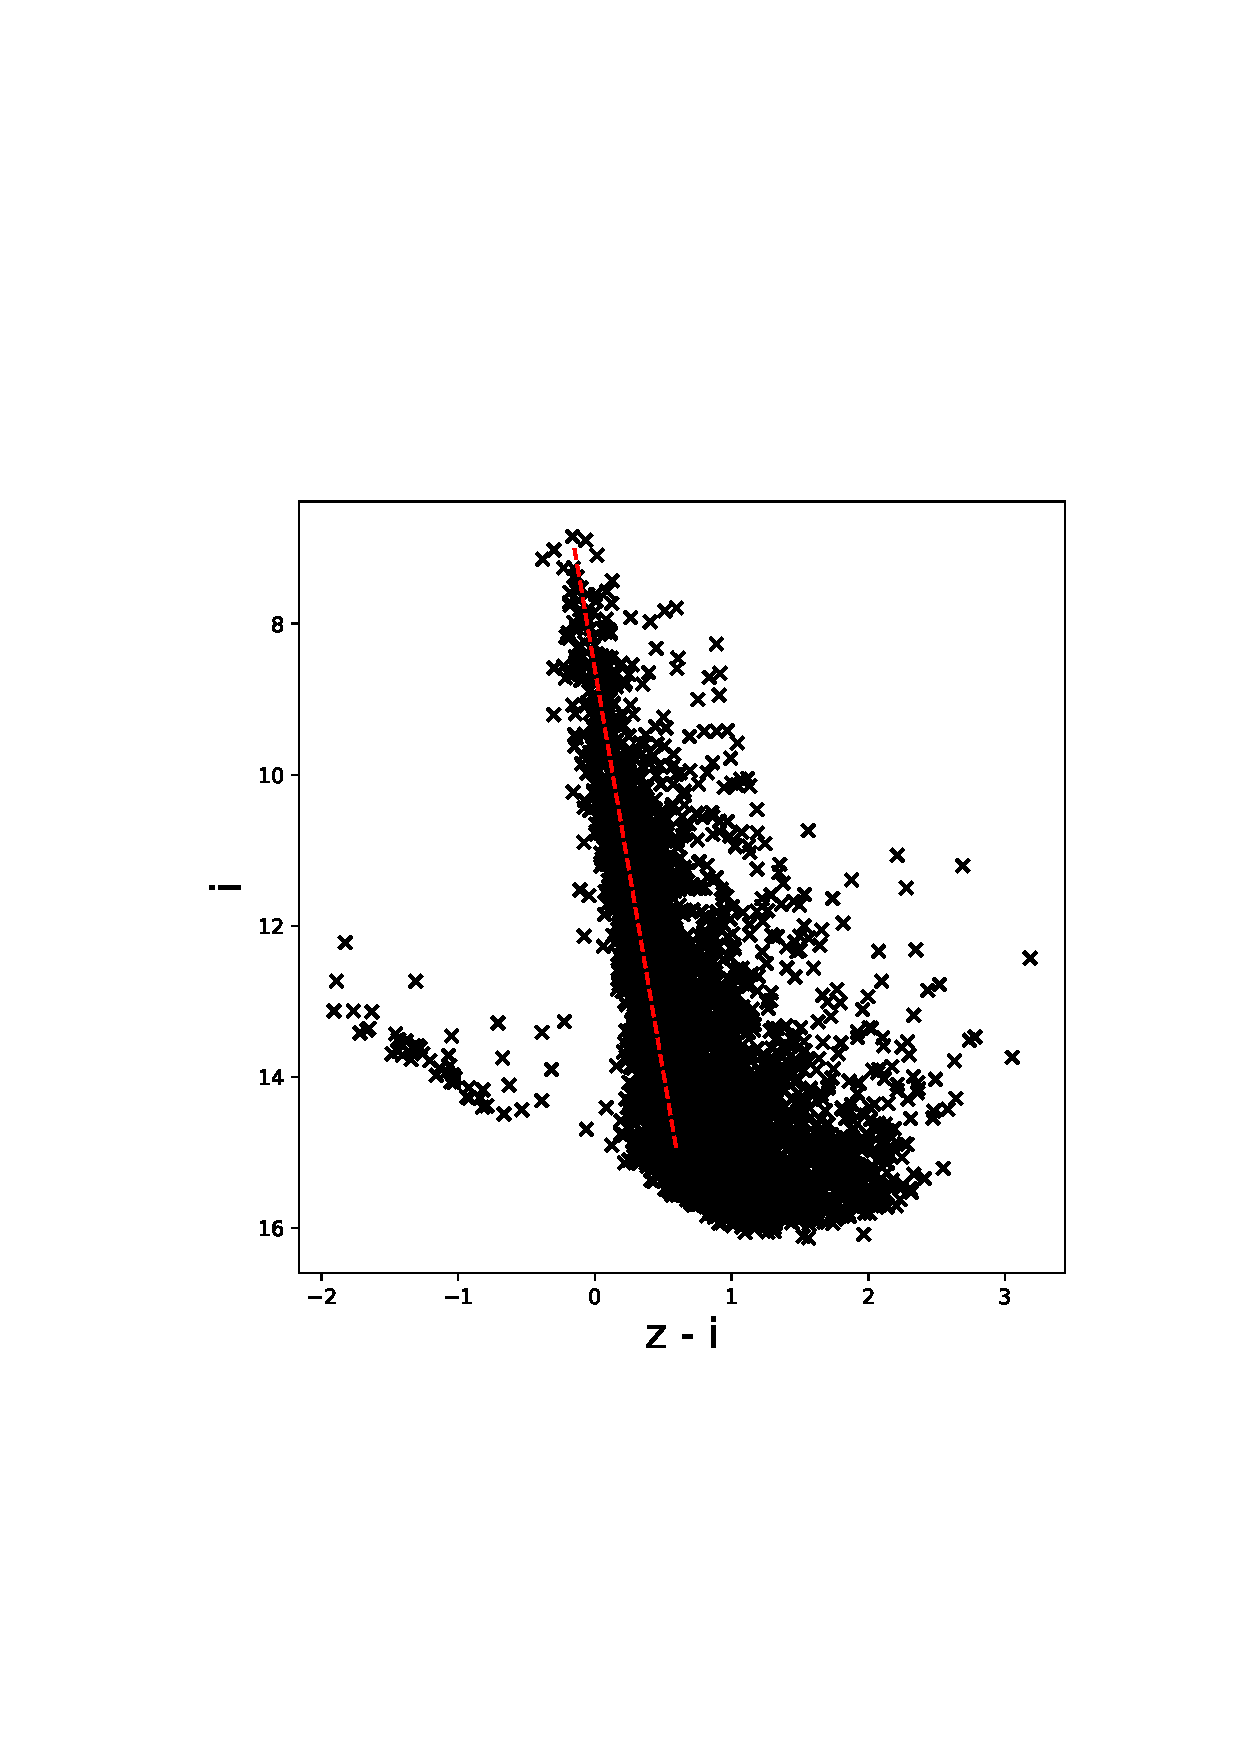
\includegraphics[width=\textwidth]{./figures/decaps/decaps_cmd.png}
    \end{subfigure}
    \caption{(Left) A 1000 x 1000 pixel subregion of the DECam survey. 
    (Right) Color magnitude diagram for the DECam image. Red dashed line highlights
    the inferred blue main-sequence stars}
    \label{fig:decaps}
\end{figure}


% With the smaller density of stars, 
% the SGD algorithm converged after only 100 epochs; 
% the fit took ten minutes. After the fit, producing the catalog 
% took only two seconds. 
% On the other hand, extrapolating the runtime of PCAT, running MCMC on the same frame
% would take on the order of day.


% \begin{figure}[tb]
%     \centering
%     \includegraphics[width=0.8\textwidth]
%     \vspace{-0.4cm}
%     \caption{A 1000 x 1000 pixel subregion of the DECAM survey. }
%     \label{fig:decaps_ex}
% \end{figure}

% \begin{figure}[tb]
%     \centering
%     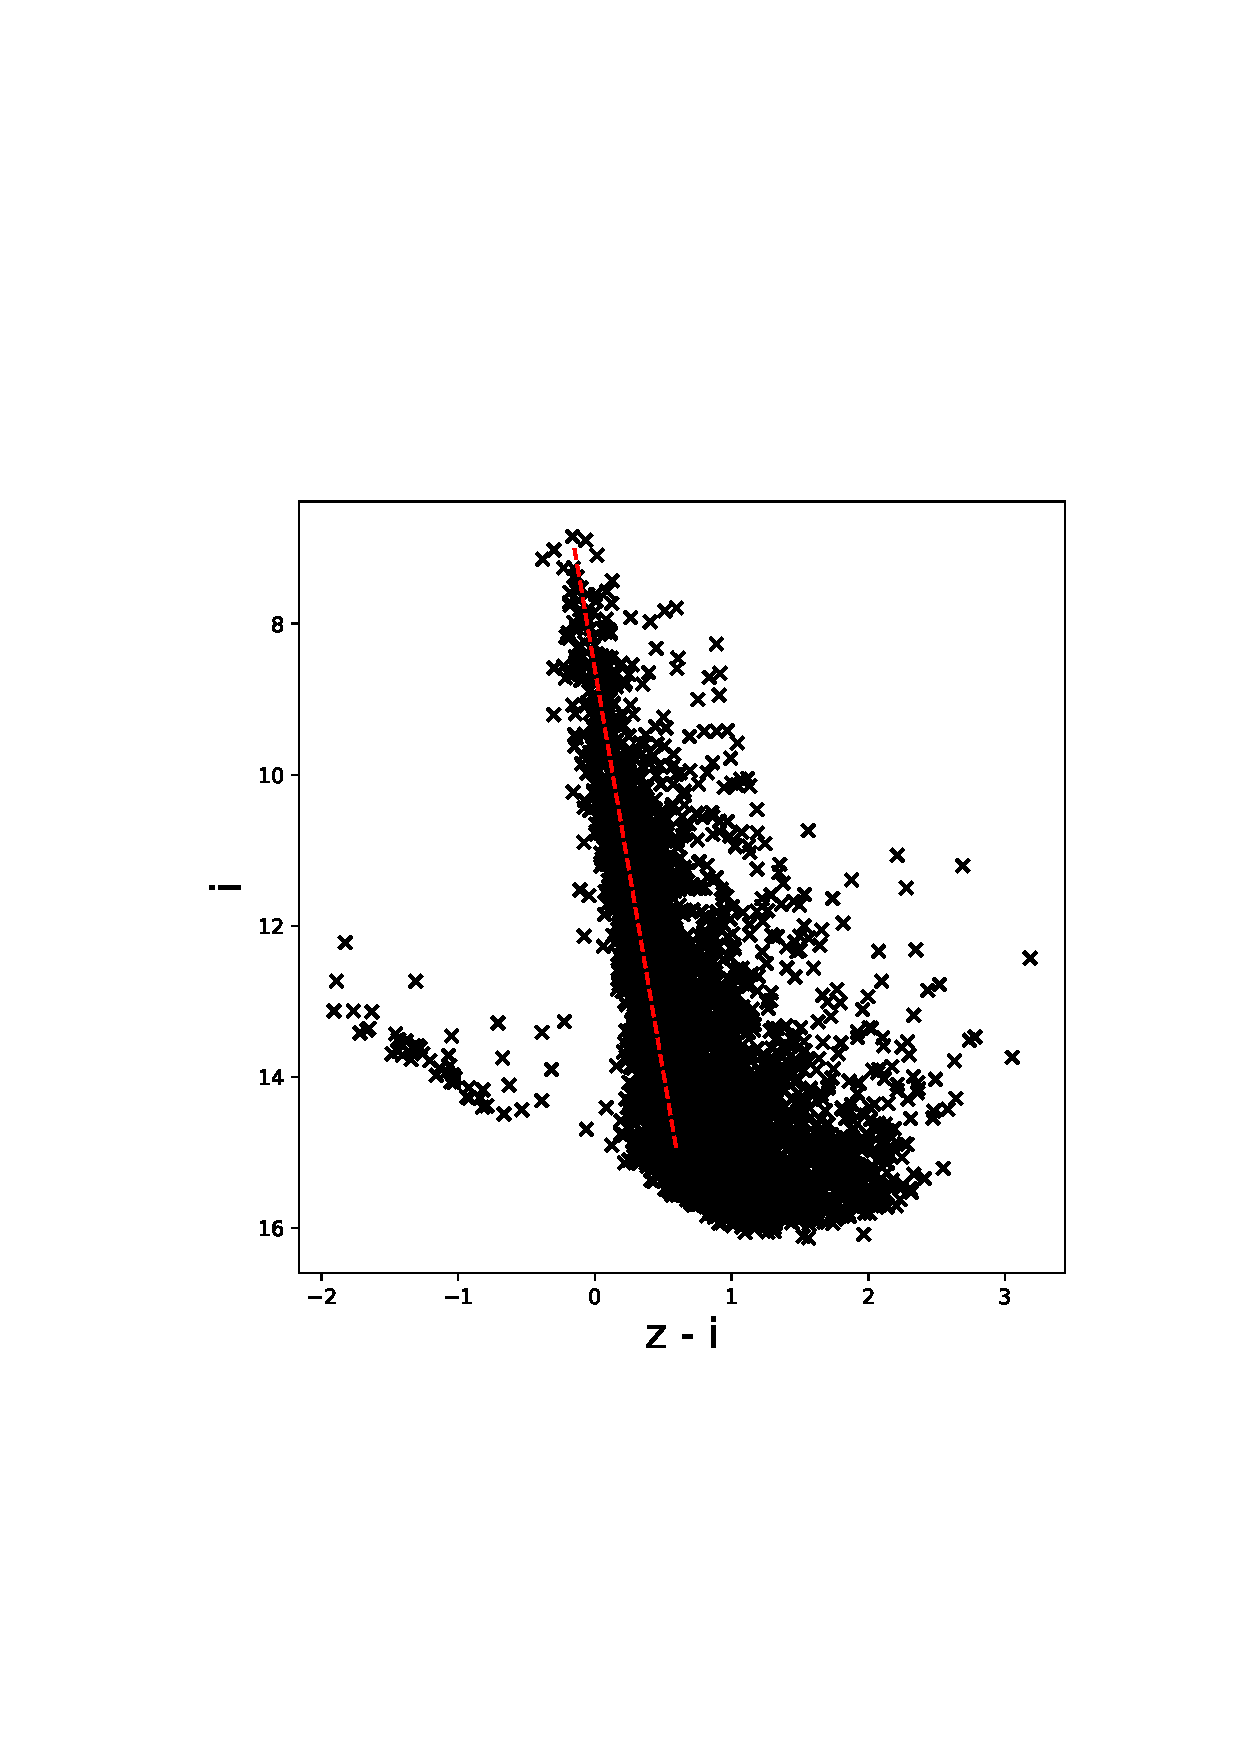
\includegraphics[width=0.4\textwidth]{./figures/decaps/decaps_cmd.png}
%     \vspace{-0.4cm}
%     \caption{Color magnitude diagram for the Decaps image. Red dashed line highlights
%     the inferred blue main-sequence stars.
%     }
%     \label{fig:decaps_cmd}
% \end{figure}


\subsection{Runtime}
\label{sec:runtime}
We ran SGD to minimize the expected forward KL
for 400 epochs; at each epoch, 200 images of size $100\times100$ pixels were sampled from the generative model.
We performed optimization with Adam~\citep{kingma2014adam}.
On a single NVIDIA GeForce RTX 2080 Ti GPU,
this fitting procedure took one hour.

After fitting the variational posterior,
computing the approximate posterior
(that is, producing the distributional parameters of the variational approximation) given either the $1000\times1000$ M2 image
or the $4000 \times 2000$ DECam image
takes less than a second. 
By comparison, the reported runtime of PCAT, which uses MCMC, is 30 minutes on a $100 \times 100$ pixel image~\citep{Feder_2019}.

The speed at inference time (which excludes training time) gives StarNet the scaling characteristics necessary for processing large astronomical surveys.
A single SDSS image is $1489 \times 2048$ pixels.
Based on the reported 30-minute runtime of PCAT for a $100\times100$ pixel subimage, we project that
the runtime to process the full image would be $30\text{ min} \times 14 \times 20 = 8400$ minutes, or almost six days.
The SDSS survey consists of nearly one million images, and thus scaling PCAT to the entire SDSS survey would be infeasible.
The upcoming LSST survey will be 300 times larger than SDSS.


On the other hand, StarNet incurs a one-time cost to fit the variational distribution with synthetic data; this cost is then amortized over a potentially large region of the sky.
Re-fitting StarNet may nonetheless be necessary when the model parameters
such as the background or PSF change---which is the case for 
large ground-based astronomical surveys, where data is collected over many nights. 
The SDSS data processing pipeline, for instance, estimates a new PSF and background
for each new frame. 
Even assuming a new StarNet refit for each SDSS frame, 
StarNet is still $100\times$ faster than PCAT. 

We can further push the scalability of StarNet by 
amortizing over a range of model parameters such as the background and PSF. 
With appropriate priors on these model parameters,
fitting StarNet using the  
expected forward KL enables it to generalize across a diverse set of images 
and further reduce the need for retraining.

